\section {Performance Testing}

\begin{frame}{Delimitations}{Jevgenijs Galaktionovs}
\begin{itemize}
    \item End-effector
    %item \textit{HIGHYAG BIMO W} is replaced by the Laser Pointer.
    \item Industrial manipulator
    %\item \textit{KUKA KR6 R700sixx} is replaced by \textit{UR5}.
    \item Focal length
    %\item Focal length is reduced from $480mm$ to $100mm$.
    \item Tolerance rate of 10\%
    %\item Tolerance rate is set to $10$\% of the tested requirement.
\end{itemize}
\begin{columns}
\column{0.4\textwidth}
\centering{
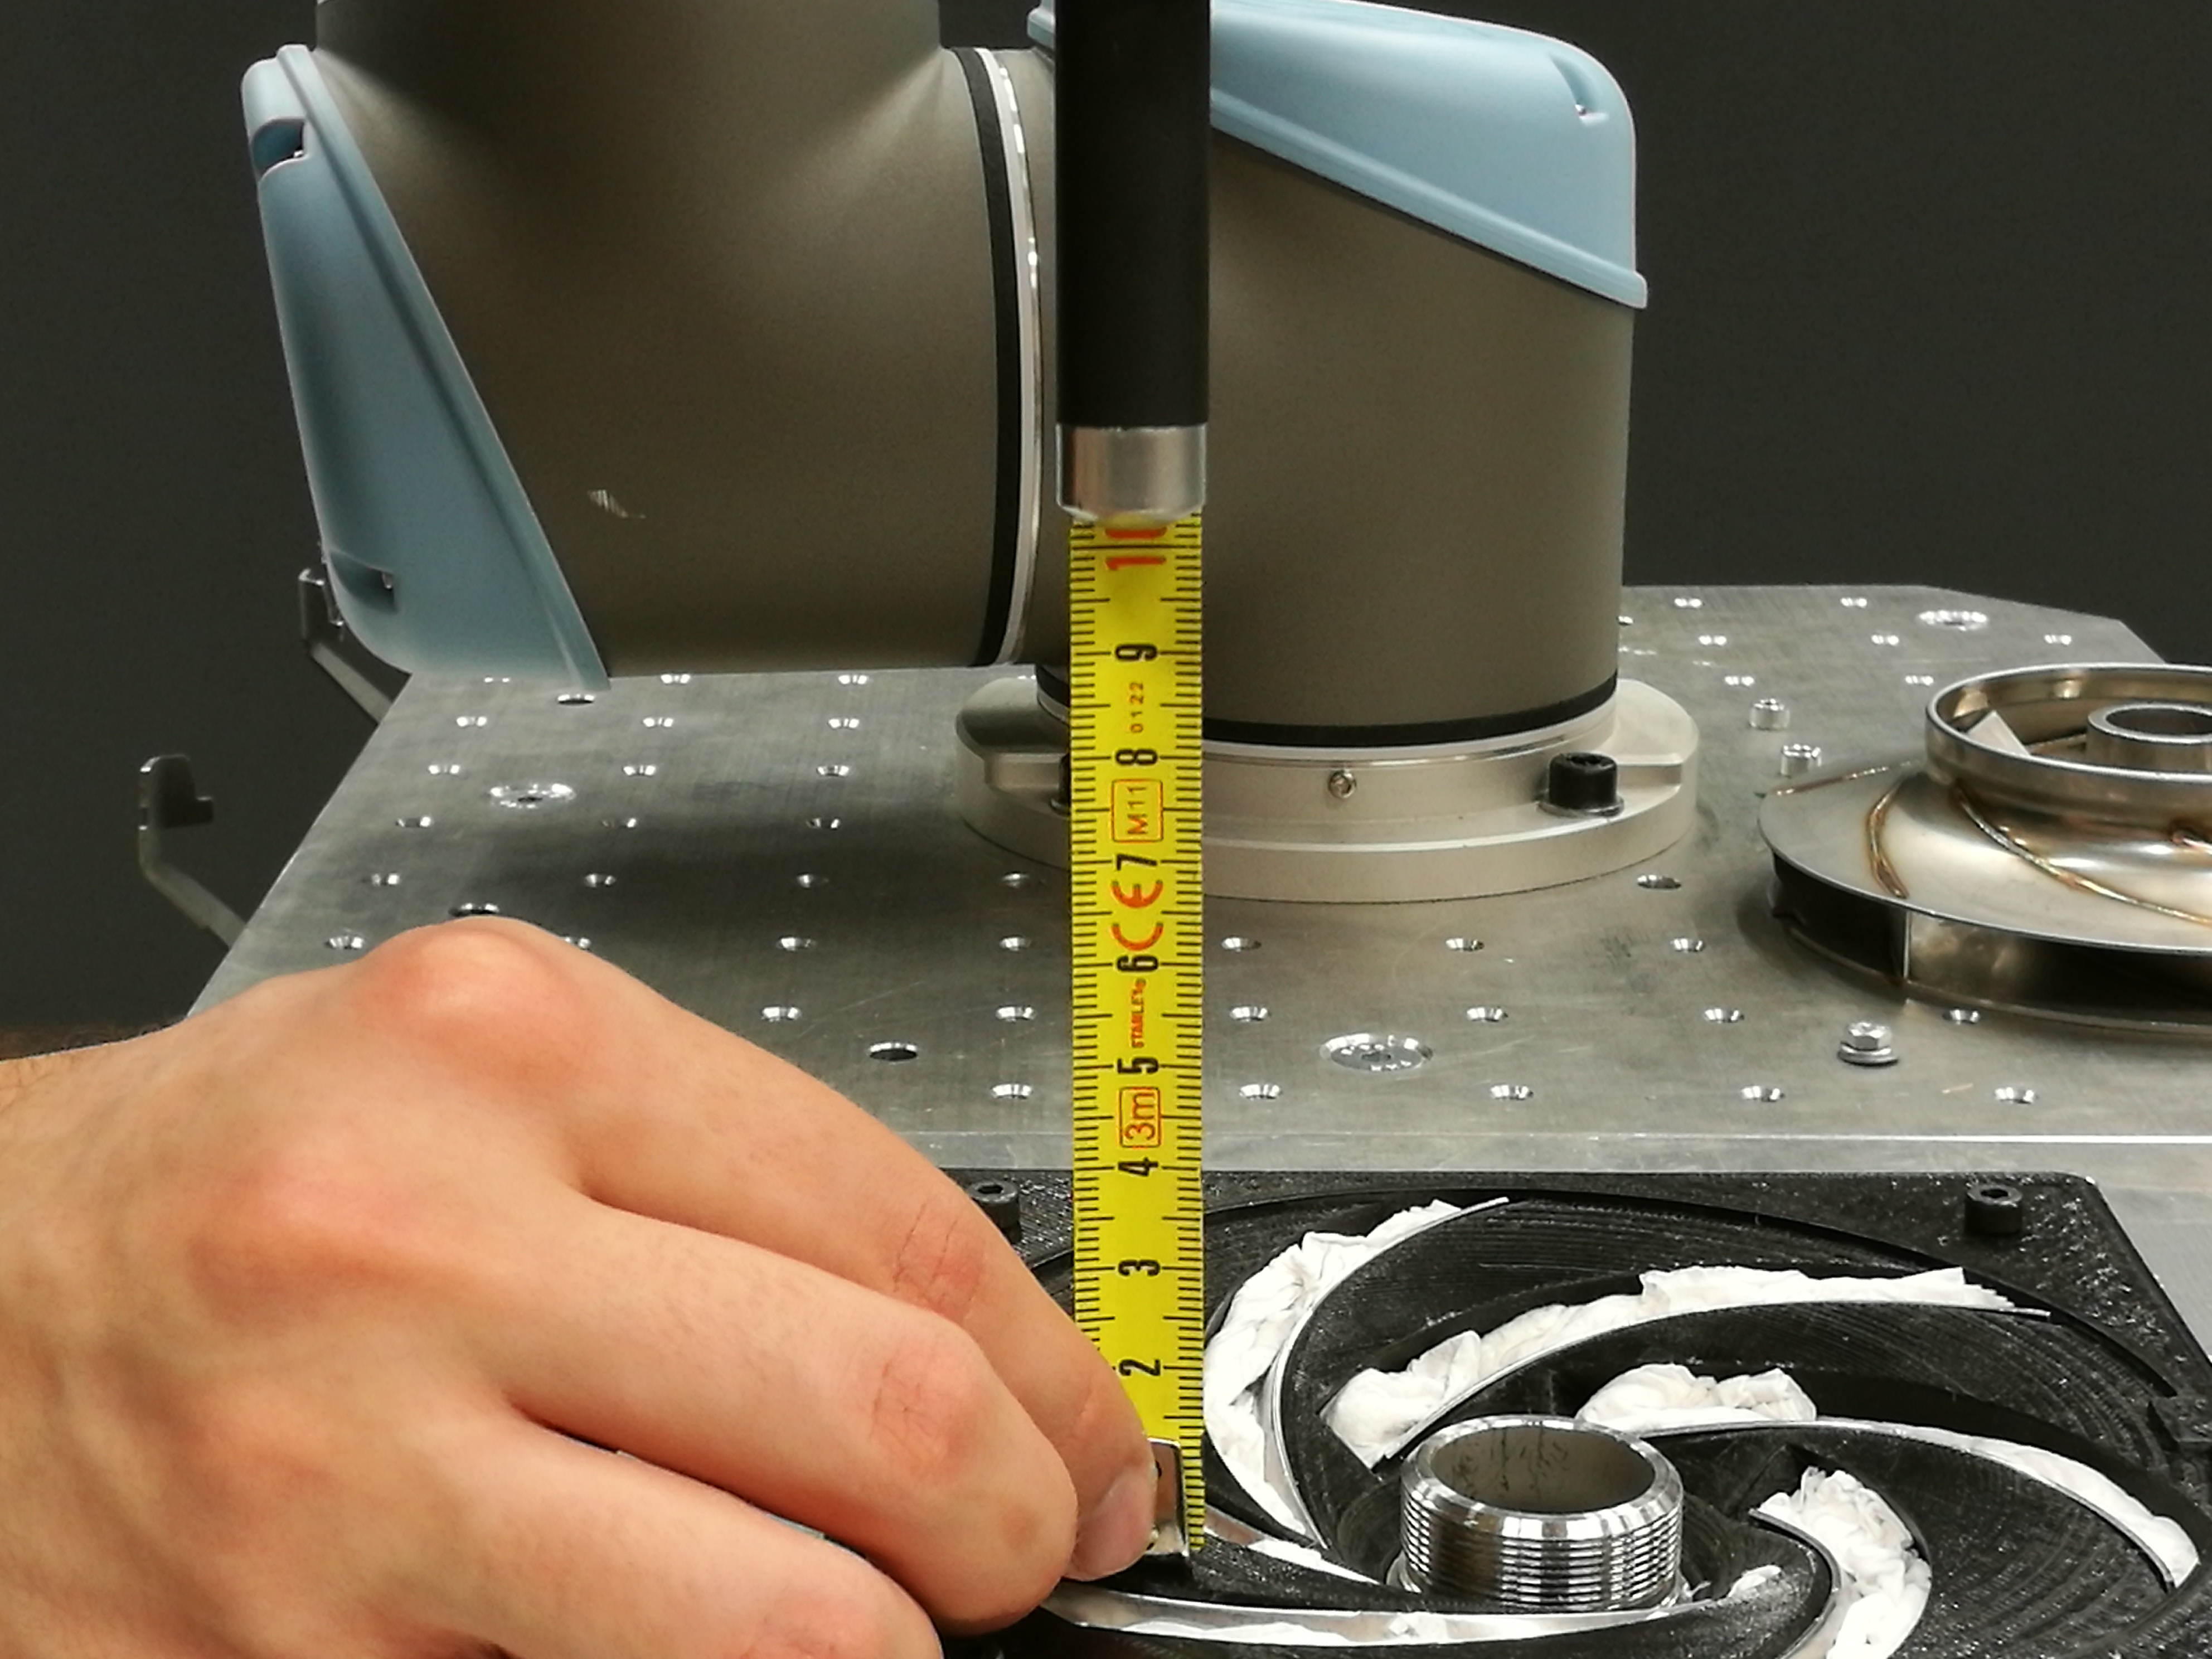
\includegraphics[width=\textwidth]{graphics/eugene/distance}}
\column{0.4\textwidth}
\centering{
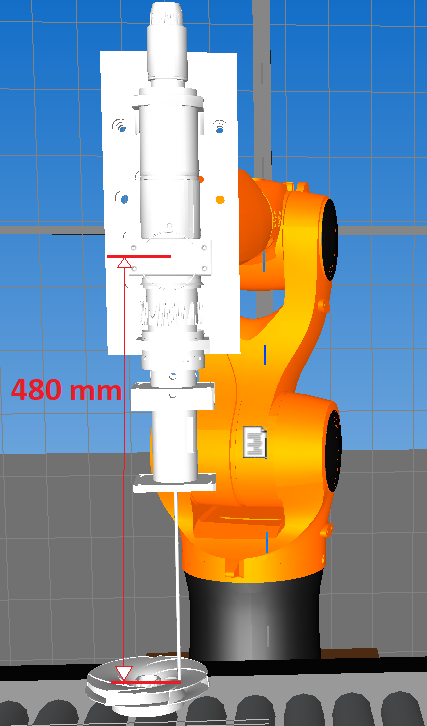
\includegraphics[scale=0.22]{graphics/eugene/focal_length480b}}

\end{columns}
\end{frame}

\begin{frame}{Laboratory Setup}
\begin{columns}
\column{0.3\textwidth}
    \begin{itemize}
    \Fontvi
        \item \textit{UR5}
        \item Table
        \item Fixture
        \item Tool Holder
        \item Laser Pointer
        \item Impeller
        \item Screens
        \item Sunography paper
        \item Light microscope
        \item \textit{Logger Pro} software

    \end{itemize}
\column{0.7\textwidth}
\centering{
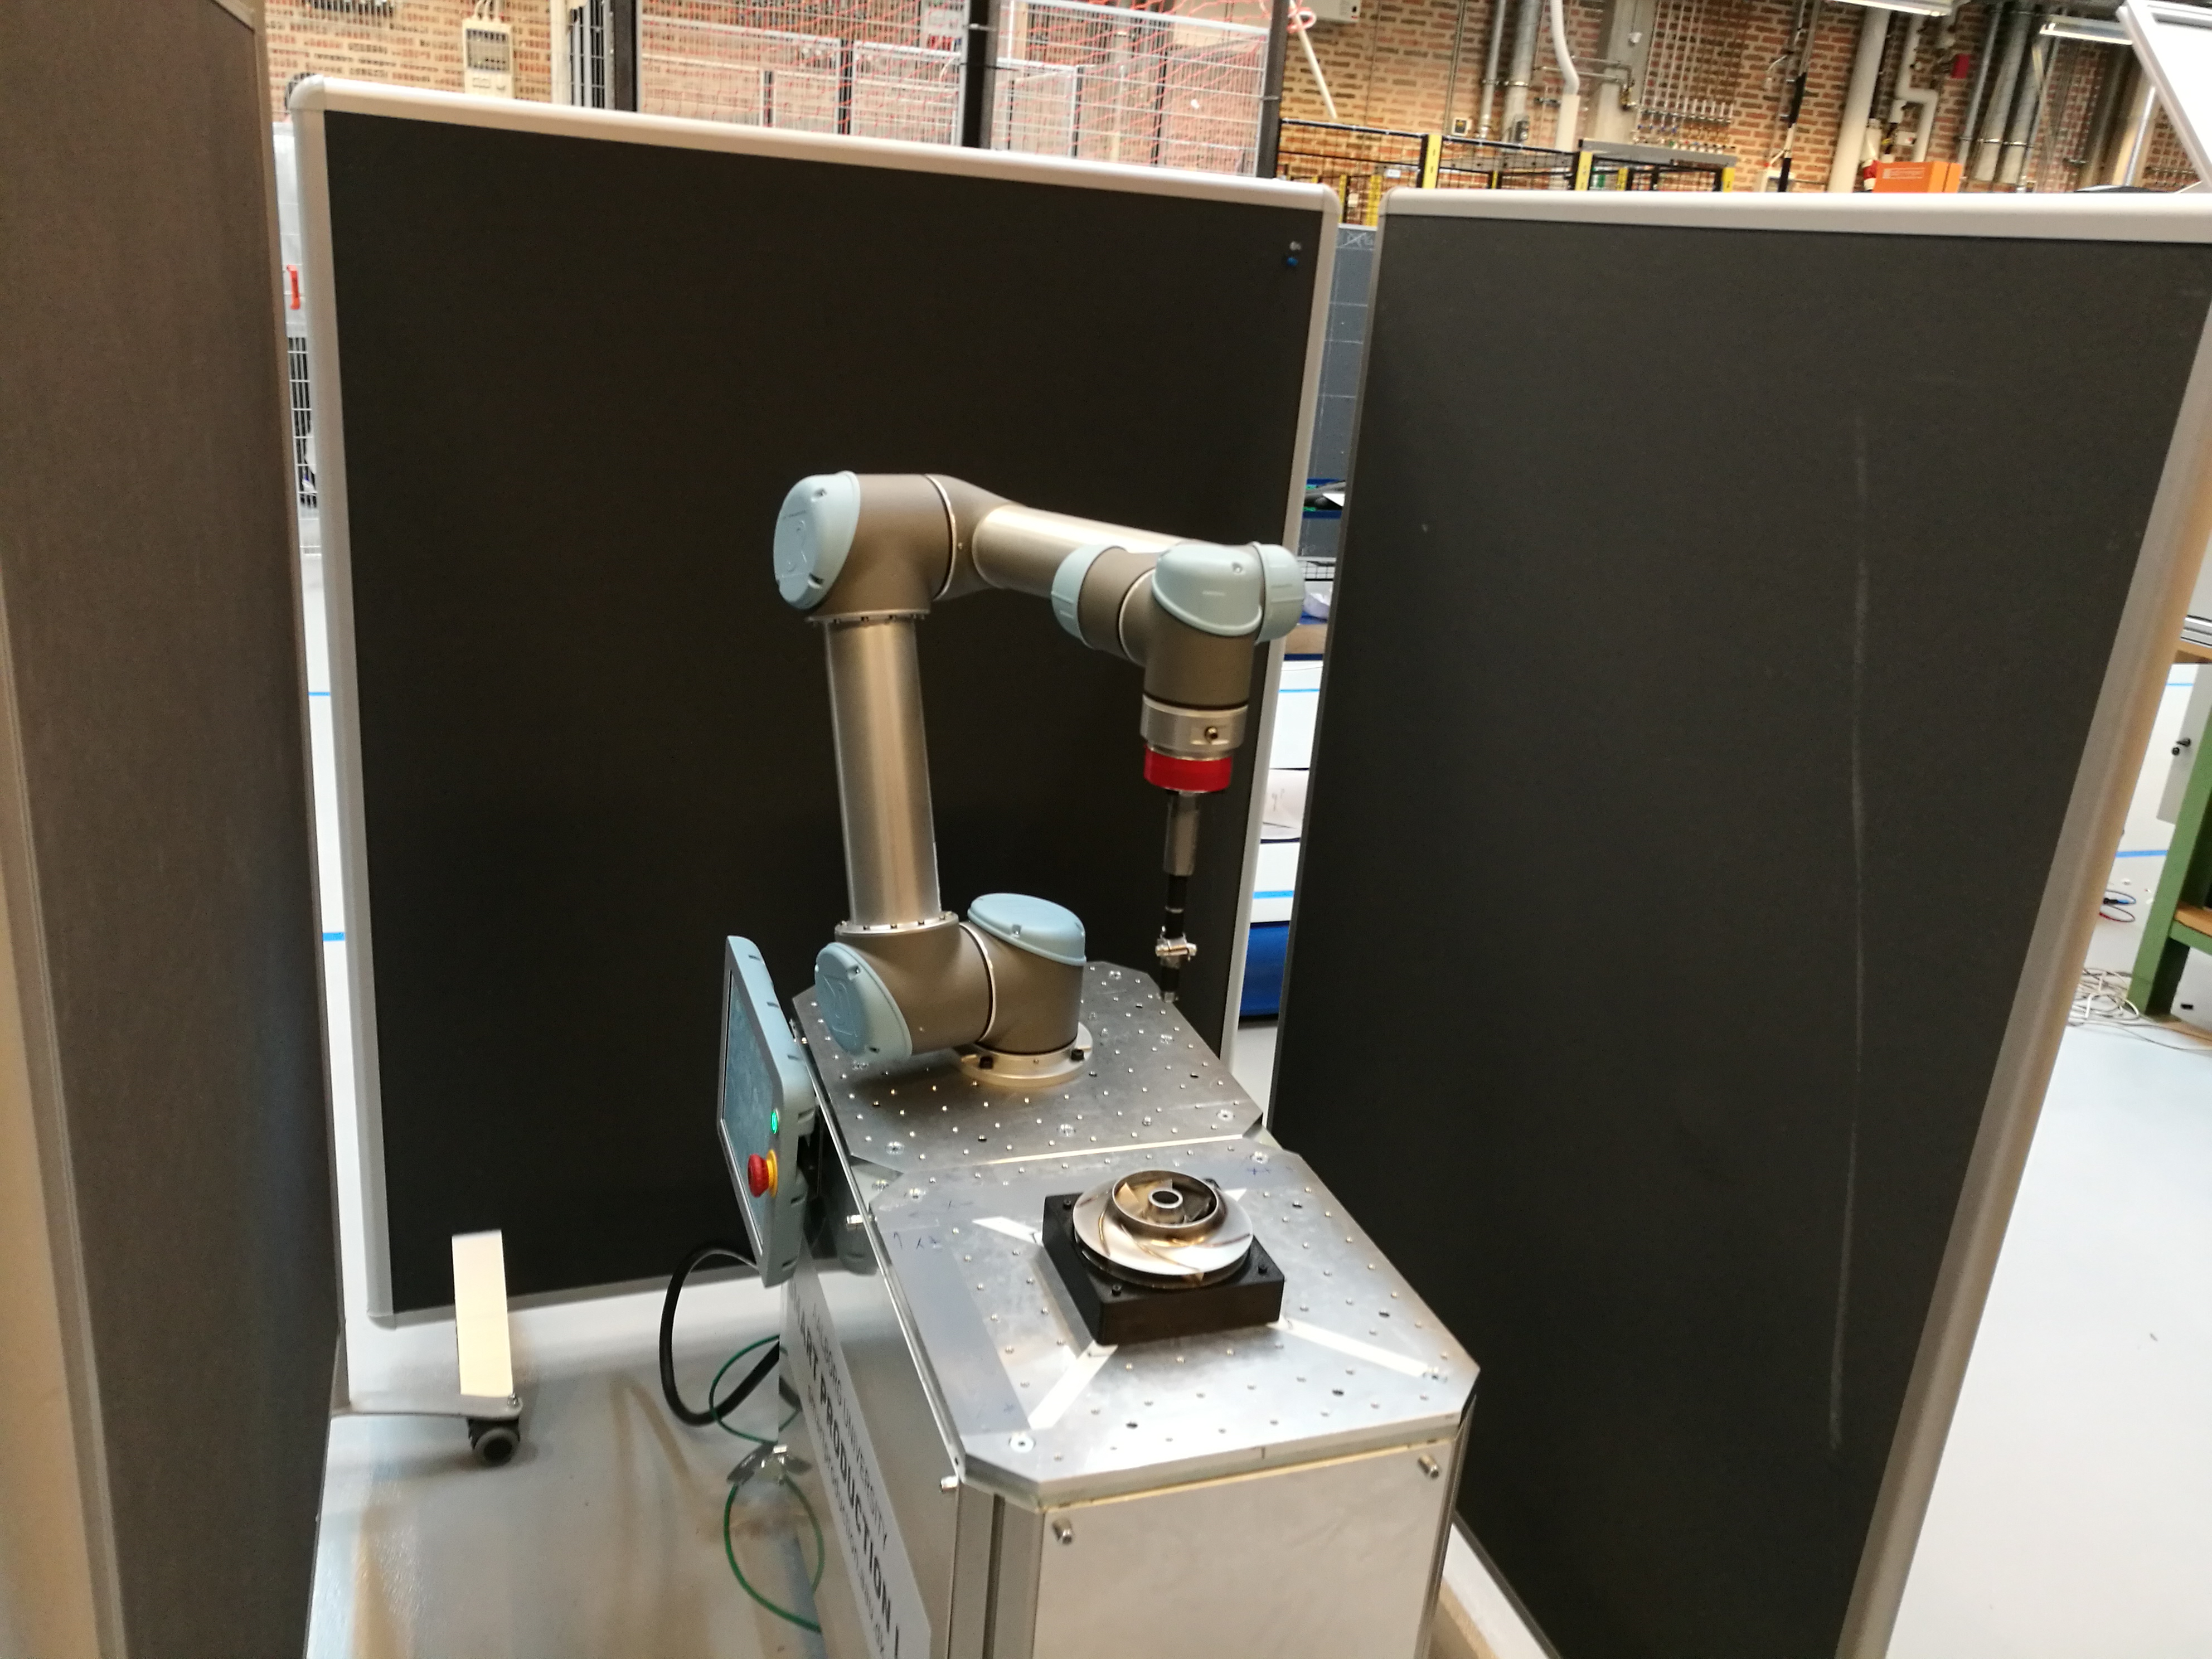
\includegraphics[scale=0.045]{graphics/eugene/lab_setup}}
\end{columns}
\end{frame}

\begin{frame}{Performance Testing}{Industrial Manipulator}
 \begin{itemize}
        \item \textbf{Purpose:} Manoeuvring of the end-effector by \textit{UR5}
        \item \textbf{Result:} Success
    \end{itemize}
    \vspace{4pt}
    \centering{
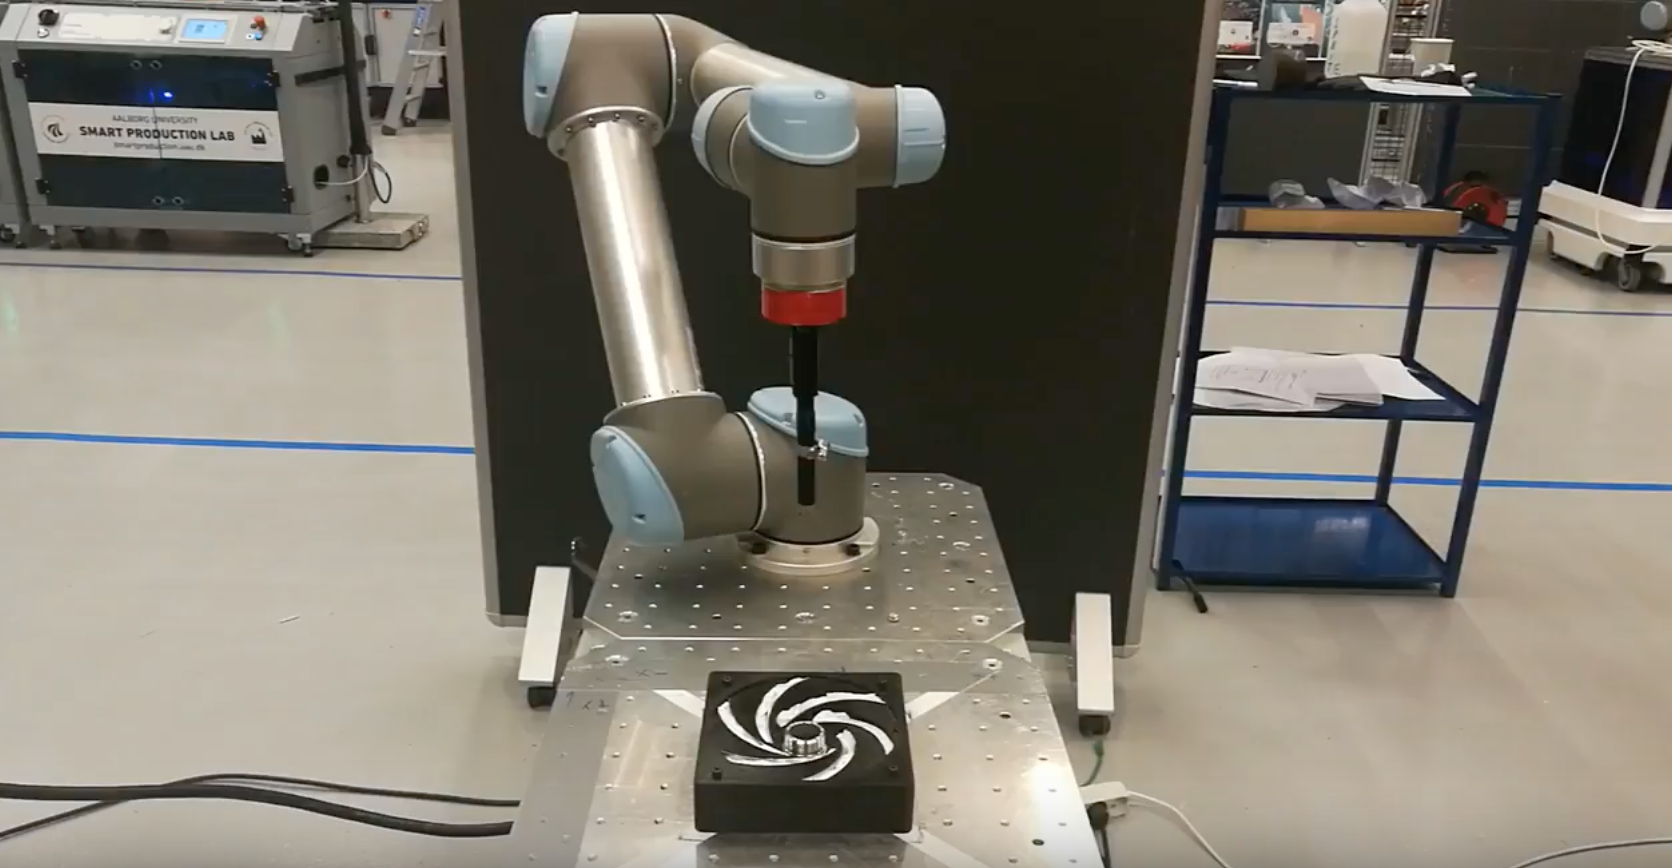
\includegraphics[scale=0.30]{graphics/eugene/jev}}
% Insert video here. If you can, with a start button or 5sec delay.
\end{frame}

\begin{frame}{Performance Testing}{Velocity}
\begin{itemize}
    \item \textbf{Purpose:} Constant velocity of $167$ $mm/s$
    %\item \textbf{Procedure:} The camera is recording the welding sequence. Video is analysed by a \textit{LoggerPro} software.
    \item \textbf{Result:} Failed
\end{itemize}
\vspace{5pt}
\begin{table}[!h]
    \centering
\begin{tabular}{cc}
    \hline
     \rowcolor{beamer@barcolor} Test Number & Average Velocity ($mm/s$)  \\
     \hline
     1 & $24.8$ \\
     \rowcolor{beamer@barcolor} 2 & $25.9$  \\
     3 & $26.1$ \\
     \hline
\end{tabular}
\end{table}
%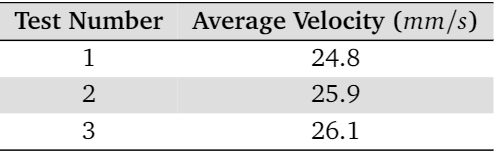
\includegraphics[scale=0.5]{graphics/eugene/velocity}}
\end{frame}

\begin{frame}{Performance Testing}{Distance}
\begin{itemize}
    \item \textbf{Purpose:} Focal length distance of $100 mm$
    %\item \textbf{Procedure:} Welding sequence is launched and stopped at a random point. Distance is measured.
    \item \textbf{Result:} Success
\end{itemize}
\vspace{5pt}
\begin{columns}
\column{0.5\textwidth}
\centering{
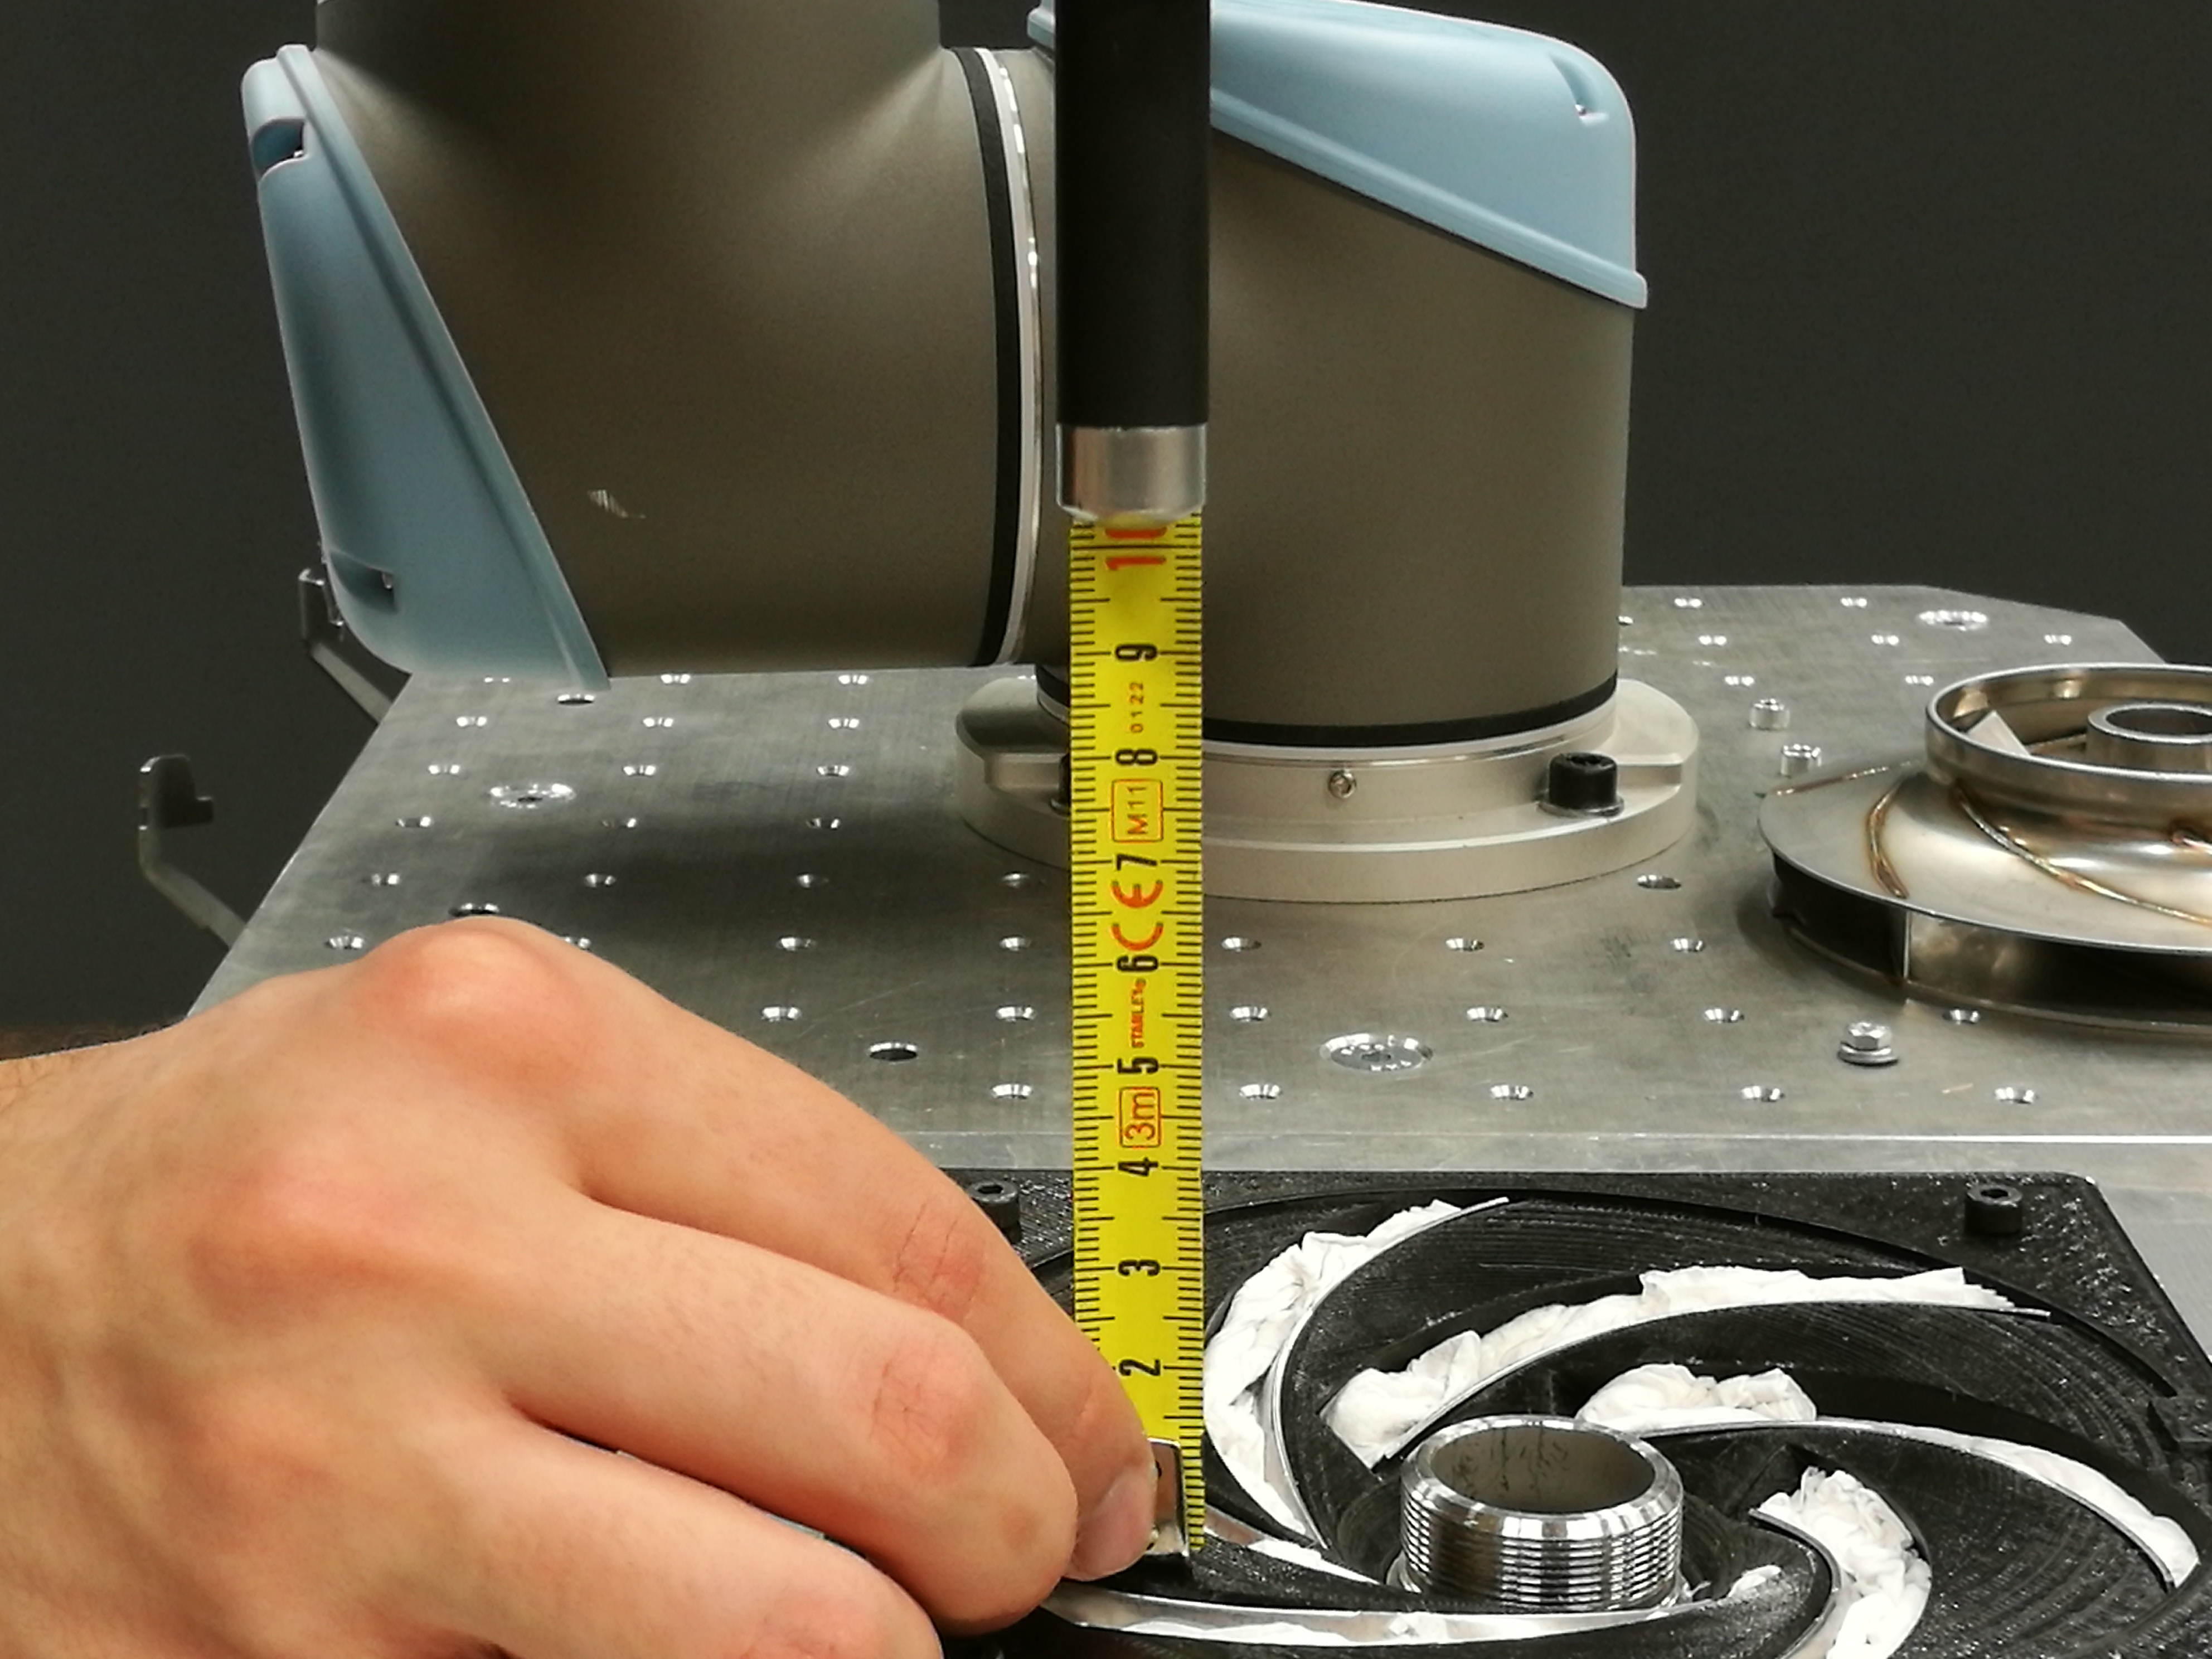
\includegraphics[scale=0.03]{graphics/eugene/distance}}
\column{0.5\textwidth} 
\begin{table}[!h]
    \centering
\begin{tabular}{m{1.5cm} m{1.7cm}}
    \hline
    \rowcolor{beamer@barcolor} 
    Test Number & Average Distance ($mm$) \\
    \hline
    $1$ & $102$  \\
    \rowcolor{beamer@barcolor} $2$ & $104$ \\
    $3$ & $103$ \\
    \rowcolor{beamer@barcolor} $4$ & $103$ \\
    $5$ & $103$ \\
    \hline
\end{tabular}
\end{table}
%\centering{
%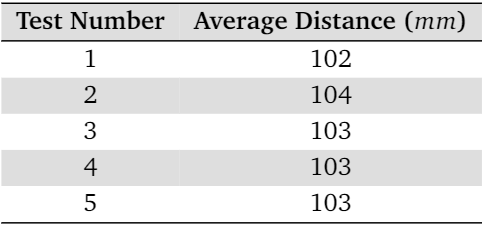
\includegraphics[width=\textwidth]{graphics/eugene/average_distances}}
\end{columns}
\end{frame}

\begin{frame}{Performance Testing}{Vane Relative Angle}
\begin{columns}
\column{0.5\textwidth}
    \begin{itemize}
        \item \textbf{Purpose:} Relative angle to vane
        \item \textbf{Result:} Success
    \end{itemize}
\column{0.4\textwidth}
\centering{
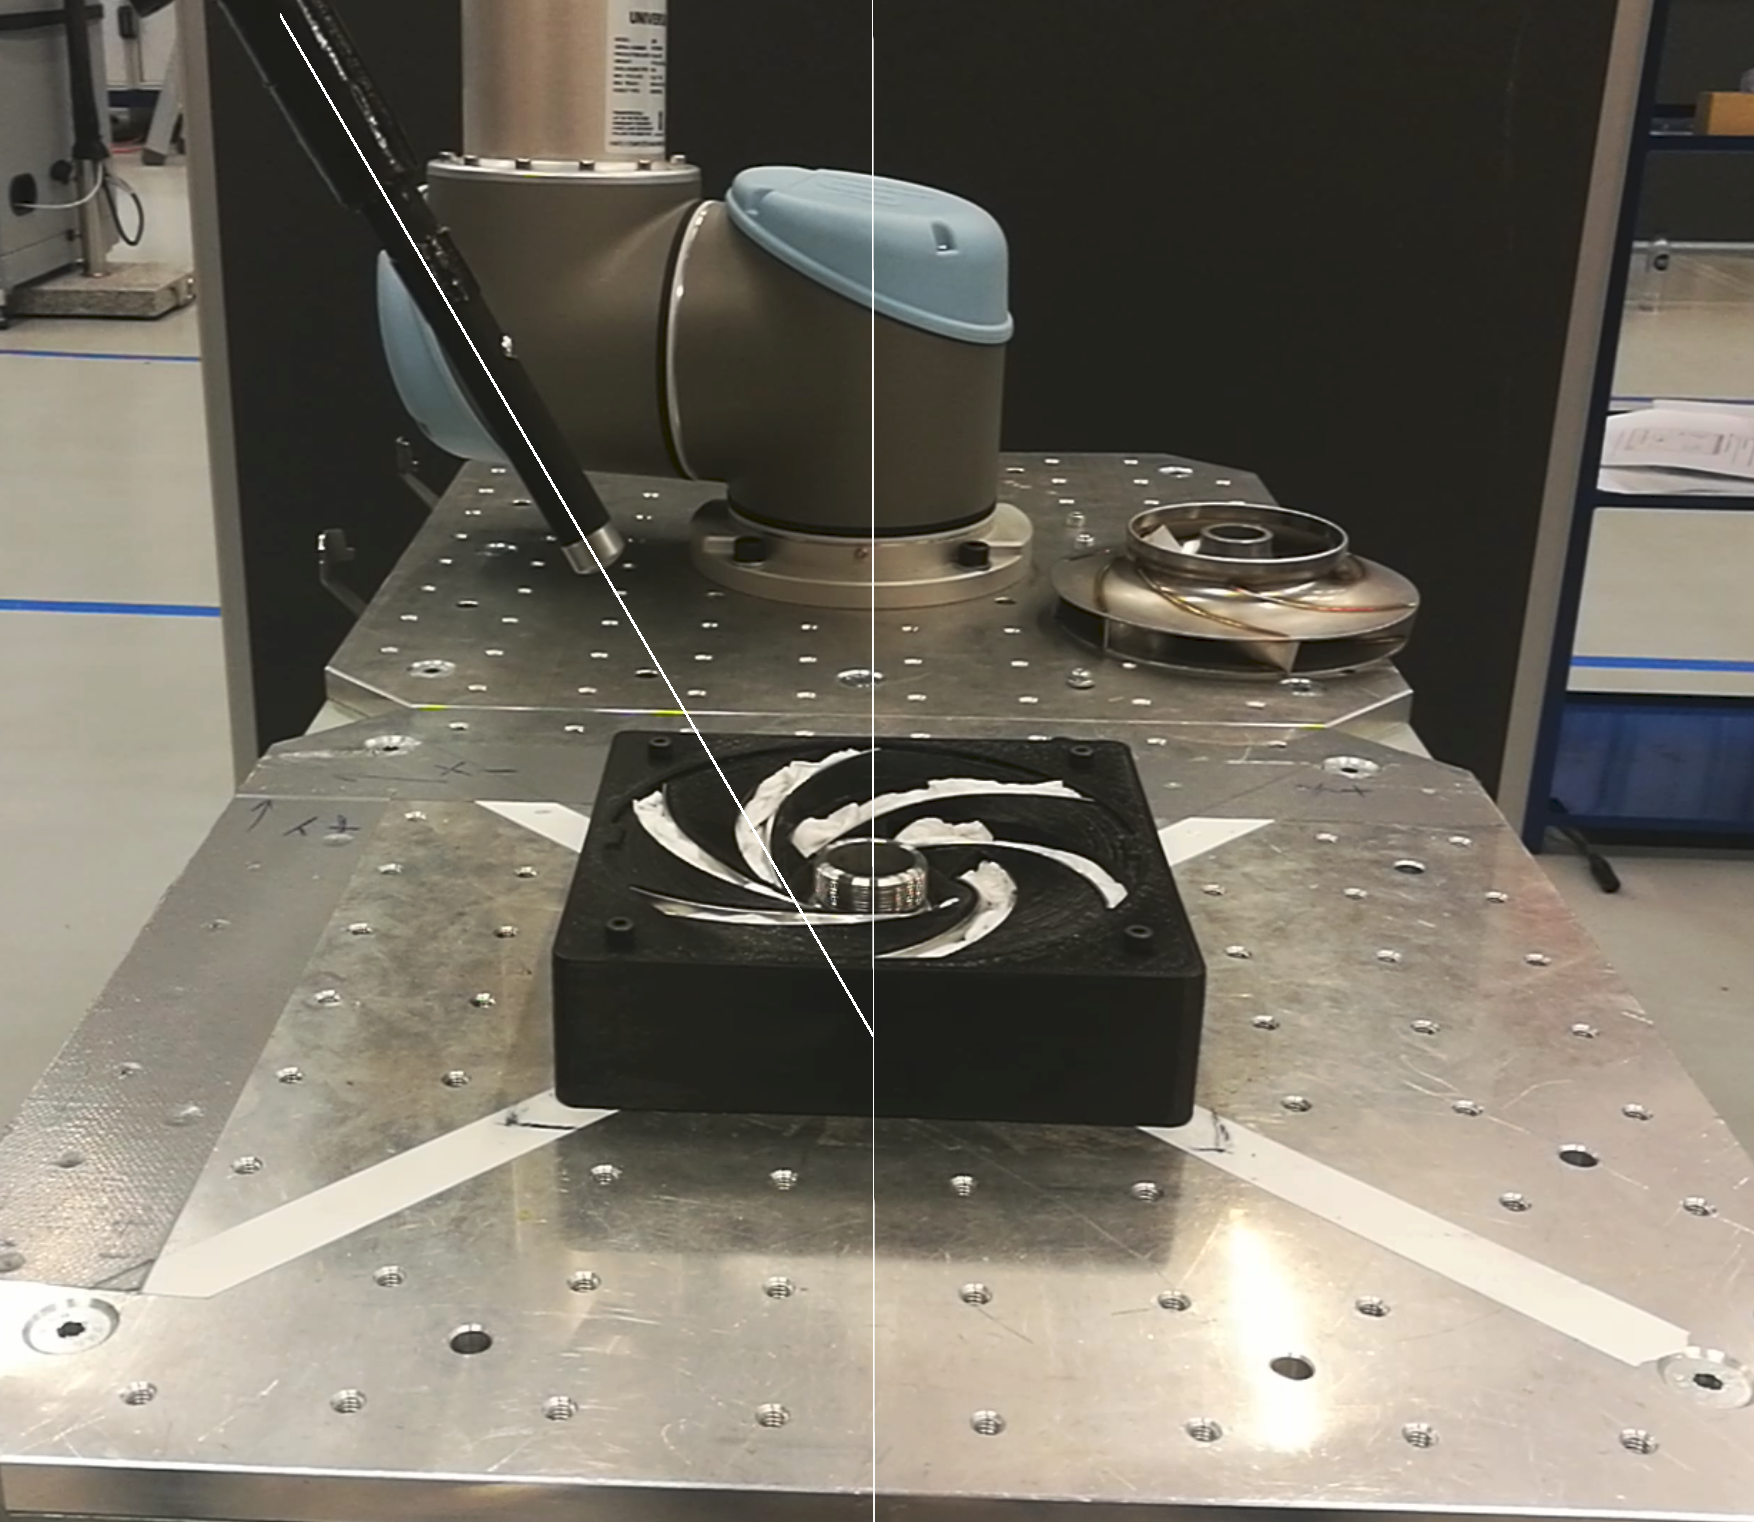
\includegraphics[width=\textwidth]{graphics/eugene/angle_picture}}
\end{columns}
\vspace{10pt}
\begin{table}[!h]
    \centering
\begin{tabular}{cc}
    \hline
     \rowcolor{beamer@barcolor} Vane Test & Average Angle ($\degree$)  \\
     \hline
      $1$ & $88.9$ \\
      \rowcolor{beamer@barcolor} $2$ & $72.4$ \\
      $3$ & $87.9$ \\
      \rowcolor{beamer@barcolor} $4$ & $97.6$ \\
      $5$ & $88.5$ \\
      \hline
\end{tabular}
\end{table}
\end{frame}



\begin{frame}{Performance Testing}{Hub Relative Angles}
\begin{columns}
\column{0.5\textwidth}
    \begin{itemize}
        \item \textbf{Purpose:} Relative angle to hub
        \item \textbf{Result:} Success
    \end{itemize}
\column{0.4\textwidth}
\centering{
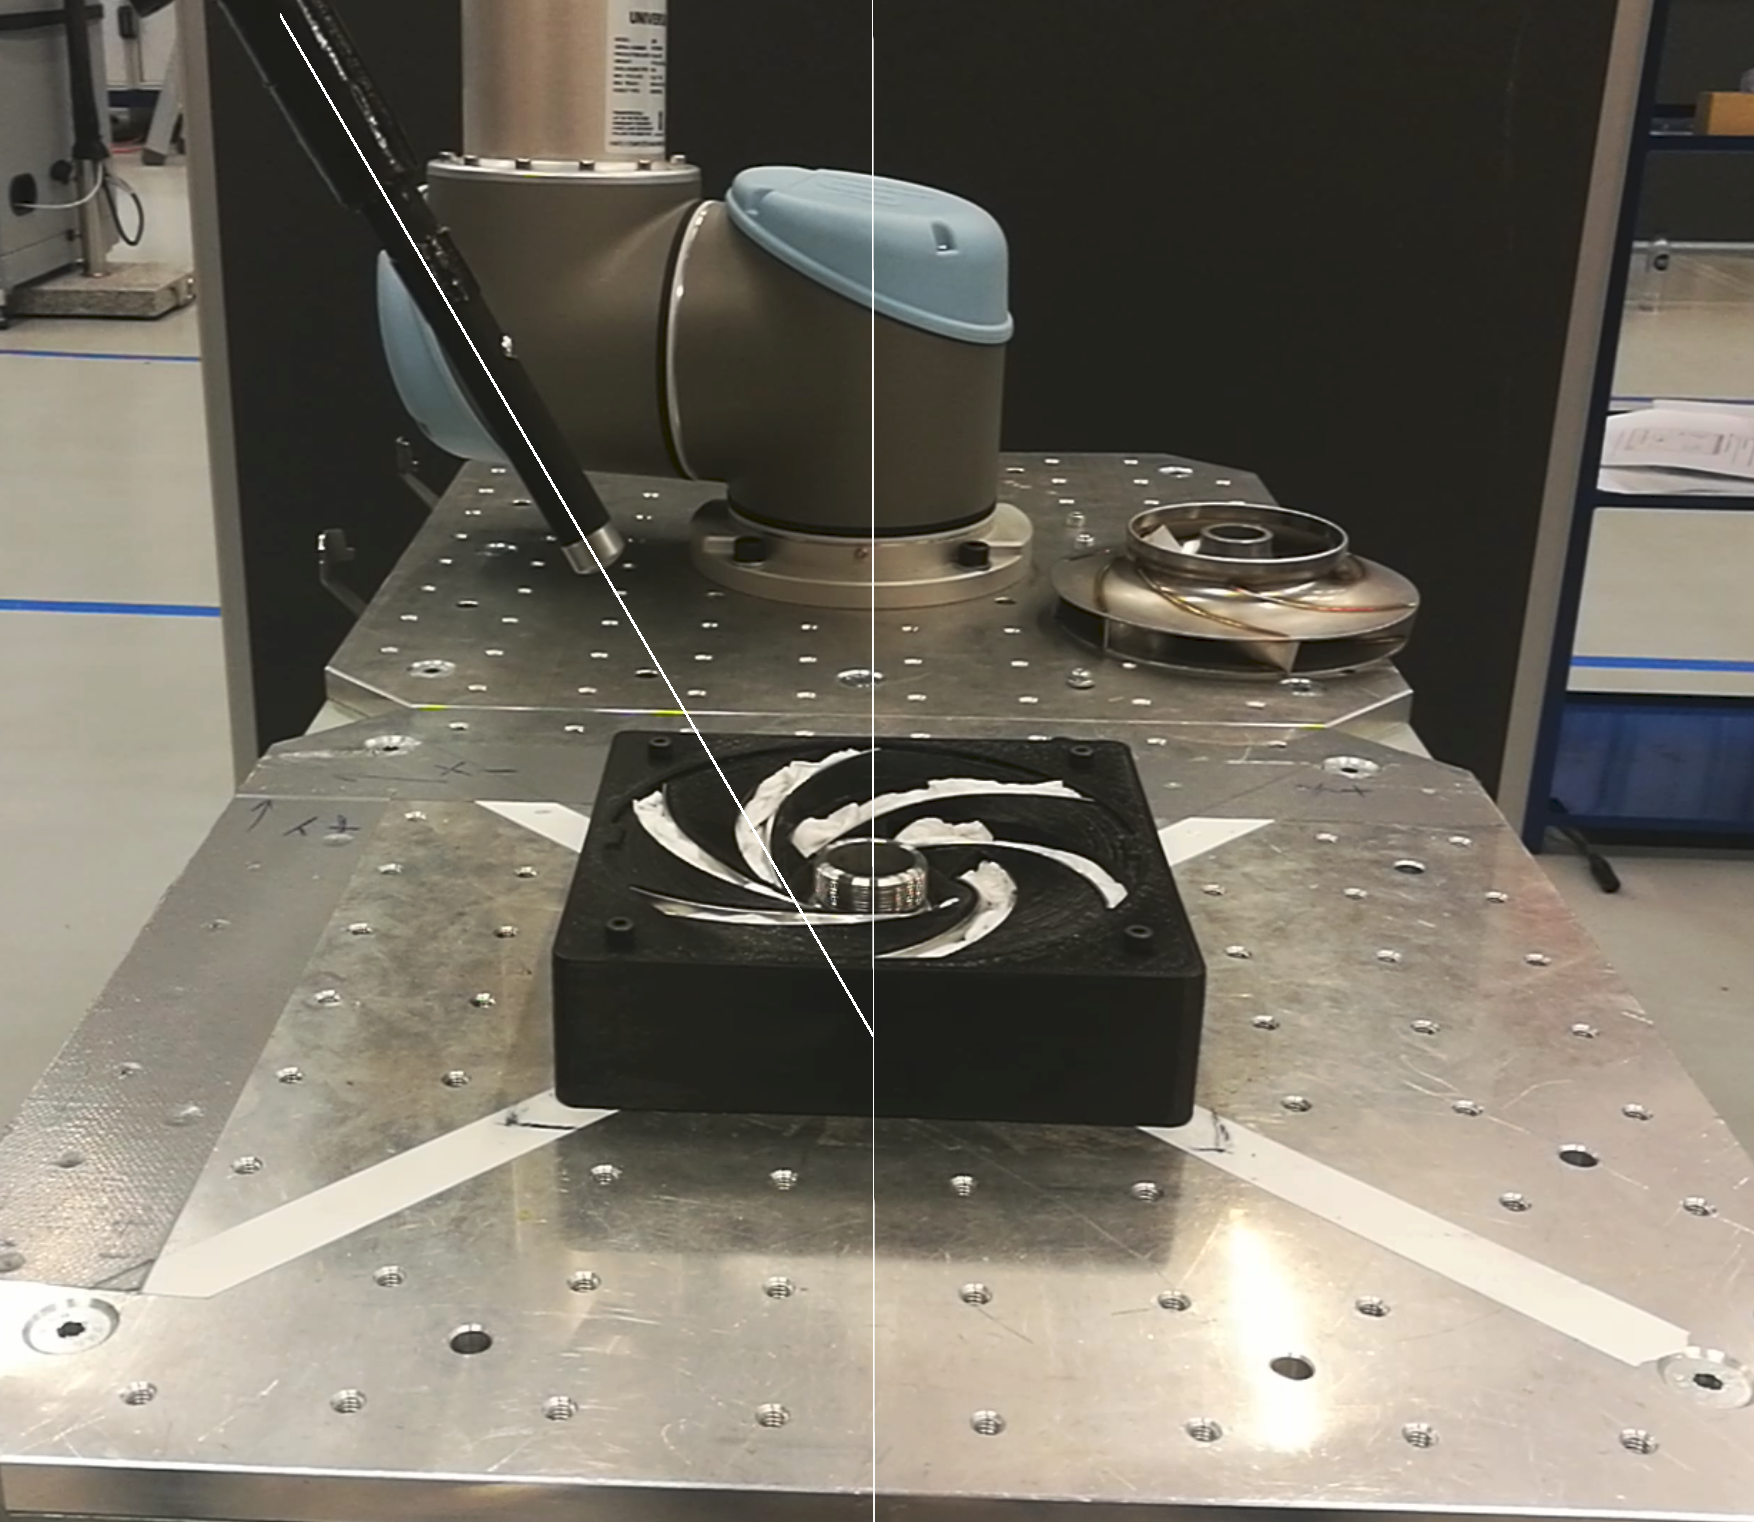
\includegraphics[width=\textwidth]{graphics/eugene/angle_picture}}
\end{columns}
\vspace{10pt}
\begin{table}[!h]
    \centering
\begin{tabular}{cc}
    \hline
     \rowcolor{beamer@barcolor} Hub Test & Average Angle ($\degree$) \\
     \hline
      $1$ & $30.3$ \\
      \rowcolor{beamer@barcolor} $2$ & $30.0$ \\
      $3$ &  $30.2$ \\
      \rowcolor{beamer@barcolor} $4$ & $30.3$ \\
      $5$ & $29.9$ \\
      \hline
\end{tabular}
\end{table}
\end{frame}



\begin{frame}{Performance Testing}{Deviation}
\begin{itemize}
    \item \textbf{Purpose:} Deviation of $0.300 mm$
    \item \textbf{Result:} Failed
\end{itemize}
\centering{
\includegraphics[scale=0.04]{graphics/eugene/microscope}}
\begin{table}[!h]
    \centering
\begin{tabular}{m{2.7cm} m{2.7cm} m{2.0cm}}
    \hline
   \rowcolor{beamer@barcolor}  \small{Minimum deviation ($mm$)} &  \small{Maximum deviation ($mm$)} &  \small{Split deviation ($mm$)} \\
    \hline
     \small{$0.100$} &  \small{$0.600$} &  \small{$0.880$}\\ 
    \hline
\end{tabular}
\end{table}
\end{frame}